% !TEX spellcheck = en-US
\documentclass[aps,prl,twocolumn,amsmath,amssymb,nobibnotes]{revtex4-1}%
\usepackage{graphicx}
\usepackage{dcolumn}
\usepackage{bm}
\usepackage{color}
\usepackage{amsmath}
\usepackage{epstopdf}
%\usepackage{caption}
%\usepackage{subcaption}
\usepackage{fancybox}
\usepackage{amsfonts}
\usepackage{amssymb}%
\usepackage{natbib}
\usepackage[toc,page]{appendix}
\usepackage[symbol]{footmisc}
%\usepackage[style=numeric-comp]{biblatex}
\setcounter{MaxMatrixCols}{30}
%\usepackage{subcaption}

\renewcommand{\cite}[1]{{[}\onlinecite{#1}{]}}

\newcommand{\s}{\sum\limits}
\newcommand{\p}{\prod\limits}
\newcommand{\pa}{\partial}
\newcommand{\il}{\int\limits}
\newcommand{\be}{\begin{equation}}
\newcommand{\e}{\end{equation}}
\newcommand{\beml}{\begin{subequations}}
\newcommand{\eml}{\end{subequations}}
\newcommand{\beq}{\begin{eqnarray}}
\newcommand{\eq}{\end{eqnarray}}
\newcommand{\ba}{\begin{array}}
\newcommand{\ea}{\end{array}}
\newcommand{\bpm}{\begin{pmatrix}}
\newcommand{\epm}{\end{pmatrix}}
\newcommand{\bc}{\begin{cases}}
\newcommand{\ec}{\end{cases}}
\newcommand{\lt}{\left}
\newcommand{\rt}{\right}
\newcommand{\n}{\nonumber}
\newcommand{\la}{\langle}
\newcommand{\ra}{\rangle}
\newcommand{\ep}{\varepsilon}
\newcommand{\dd}{\displaystyle}
\newcommand{\bs}{\boldsymbol}
\newcommand{\h}{^\dagger}
\newcommand{\ph}{^{\phantom{\dagger}}}
\newcommand{\one}{\openone}
\newcommand{\ut}{\underaccent{\tilde}}
\newcommand{\ul}{\underaccent{\bar}}
\newcommand{\up}{\uparrow}
\newcommand{\dn}{\downarrow}
\DeclareMathOperator{\var}{var}
\DeclareMathOperator{\tr}{Tr}
\DeclareMathOperator{\diag}{diag}
\DeclareMathOperator{\im}{Im}
\DeclareMathOperator{\re}{Re}
\DeclareMathOperator{\ctg}{cotan}
\DeclareMathOperator{\arcsh}{arcsinh}
\DeclareMathOperator{\csch}{csch}
\DeclareMathOperator{\rot}{rot}

\newcommand{\AQ}[1]{\textbf{\textcolor{red}{{#1}}}}

\begin{document}
\title{Ultrafast Control of Spin-Spin Interactions in Two-Dimensional Magnets}

\author{Juan M. Losada}
\affiliation{Center for Quantum Spintronics, Department of Physics, Norwegian University of Science and Technology, NO-7491 Trondheim, Norway}
\author{Arne Brataas}
\affiliation{Center for Quantum Spintronics, Department of Physics, Norwegian University of Science and Technology, NO-7491 Trondheim, Norway}
\author{Alireza Qaiumzadeh}
%\thanks{Corresponding author: alireza.qaiumzadeh@ntnu.no}
\affiliation{Center for Quantum Spintronics, Department of Physics, Norwegian University of Science and Technology, NO-7491 Trondheim, Norway}
%\affiliation{Institute for Advanced Studies in Basic Science (IASBS), Zanjan, Iran}

\begin{abstract}
Light provides ultrafast, direct and non-thermal control of exchange and Dzyaloshinskii-Moriya interactions. We consider two-dimensional honeycomb lattices described by the Kane-Mele-Hubbard model at half-filling and in the strongly correlated limit, i.e., the Mott insulator regime of a canted antiferromagnet. Based on the Floquet theory, we demonstrate that changing the amplitude and frequency of polarized laser pulses, tunes the amplitude, the sign and even the ratio between these two spin interactions. Furthermore, the renormalizations of the spin interactions are helicity independent. Our results pave the way for ultrafast optical manipulation of spins in recently discovered two-dimensional magnetic materials.
\end{abstract}

\date{\today}
\maketitle

\textit{Introduction}.--- The discovery of all-optical control of the order parameters in antiferromagnetic (AFM) and ferromagnetic (FM) materials by ultrashort, intense and high-frequency laser pulses has transformed spintronics to a new era of ultrafast magnetism \cite{kimel2005ultrafast,Rasing}. 
Recent experiments have shown that laser pulses can directly modify the amplitude and sign of the exchange interaction, the strongest spin interaction in magnetically ordered systems \cite{2018Natur.553..481G,Mikhaylovskiy2015,Perakis,PhysRevLett.93.197403}. Although the underlying microscopic mechanism remains unclear, there have been many attempts to uncover its origins.   
Recently, it has been theoretically proposed that the non-thermal optical modification of exchange interaction is possible through direct coupling between electric field of light and spins \cite{PhysRevLett.113.057201,PhysRevLett.115.075301,Mentink2015,PhysRevLett.118.097701,Stepanov2017,Kitamura,MentinkReview,Barbeau2018}.
In magnetic systems with broken inversion symmetry there is an antisymmetric exchange interaction between spins that breaks the chiral symmetry called the Dzyaloshinskii-Moriya interaction (DMI) \cite{dzyaloshinsky1958, moriya1960,Alireza-DMI1, Alireza-DMI2}. Although this interaction is much weaker than the exchange interaction, its presence has important consequences in magnetic materials and causes weak ferromagnetism in AFM materials \cite{dzyaloshinsky1958, moriya1960}, topological objects like chiral skyrmions \cite{2009Sci...323..915M,2017NatRM...217031F,AlirezaSk1, AlirezaSk2} and chiral domain walls \cite{Thiaville_2012,Parkin,AlirezaSW}, and exotic phase of topological magnon insulators \cite{Owerre2016, Elyasi2018, Chen2018, Owerre1, Owerre2}. The ratio between these two interactions controls the tilting angle of the canted spins. Finding a mechanism to tune this ratio enables new phenomena in ultrafast spin dynamics and switching \cite{Mikhaylovskiy2015,Mentink2015,Stepanov2017,Kitamura}.

Another recent important breakthrough in spintronics is the discovery of two-dimensional (2D) van der Waals AFM and FM materials with metallic, semiconducting and insulating band structures \cite{2D1,2D2}. The advantage of low dimensionality and magnetic order in the same material enables novel spintronics devices with exceptional performances.

In this Letter, we show that intense and high-frequency laser pulses can change the spin-spin interactions and the ratio between the exchange interaction and the DMI dramatically in a wide class of 2D magnetic materials described by the Kane-Mele-Hubbard model.


\textit{Model Hamiltonian}.---
Electrons in a 2D planar honeycomb lattice in the presence of electron-electron interactions can be described by the Kane-Mele-Hubbard model \cite{Kane2005,PhysRevLett.107.010401,PhysRevLett.106.100403,PhysRevB.82.075106,PhysRevB.84.235149,Griset2012,Auerbach}.
The Hamiltonian in the absence of external perturbations is the sum of the kinetic term $\hat{\mathcal{H}}_t$, the intrinsic SOI $\hat{\mathcal{H}}_{\text{SOI}}$ and the Coulomb interaction between the electrons modelled by the extended Hubbard interaction $\hat{\mathcal{H}}_{\text{int}}$,
\begin{equation}
\label{MKMH}
\hat{H}_0 = \hat{\mathcal{H}}_{\text{K}} + \hat{\mathcal{H}}_{\text{SOI}} + \hat{\mathcal{H}}_{\text{int}},
\end{equation}
where
\begin{align}
&\hat{\mathcal{H}}_{\text{K}} = - t_{1}\sum_{\langle i,j \rangle, \tau} \hat{c}_{i \tau}^\dagger \hat{c}_{j \tau} - t_{2}\sum_{\langle \langle i,j \rangle \rangle, \tau} \hat{c}_{i \tau}^\dagger \hat{c}_{j \tau}, \label{Ht} \\
&\hat{\mathcal{H}}_{\text{SOI}}  = i \Delta \sum_{\langle \langle i,j \rangle \rangle, \tau,\tau'} \nu_{ij}\sigma^z_{\tau, \tau'}\hat{c}_{i \tau}^\dagger \hat{c}_{j \tau'} \label{Hsoi}, \\
&\hat{\mathcal{H}}_{\text{int}} = U_{00}\sum_{i=1} \hat{n}_{i\uparrow}\hat{n}_{i\downarrow} + \frac{1}{2}\sum_{\langle i,j \rangle, \tau \tau'} V_{ij}\hat{n}_{i\tau}\hat{n}_{j\tau'} \label{Hint}.
\end{align}
Here $\langle\cdot\rangle$ and $\langle\langle\cdot\rangle\rangle$ denote, respectively, nearest neighbors (NN) and next-nearest neighbours (NNN), $\hat{c}_{i \sigma}^\dagger$ ($ \hat{c}_{i \sigma}$) are fermionic creation (annihilation) operators for an electron on site $i$ and spin state $\tau=\{\uparrow,\downarrow\}$, $t_1$ and $t_2$ are NN and NNN hopping amplitudes, $\Delta$ is the intrinsic SOI parameter, $\nu_{ij}=\pm 1$ depending on whether the electron traversing from $i$ to $j$ makes a right ($+1$) or a left turn ($-1$), $\sigma^{z}$ is the $z$-component of Pauli matrices $\bm{\sigma}$, $U_{00}$ and $V_{ij}$ are the on-site and NN Coulomb interactions.
The presence of the intrinsic NNN SOI, Eq. (\ref{Hsoi}), reduces the $\mathrm{SU}(2)$ symmetry of the original Hubbard model to the $\mathrm{U}(1)$ spin group. In buckled noncoplanar honeycomb lattices and systems with structural inversion asymmetry, the presence of, respectively, NNN and NN Rashba SOIs, further reduces the symmetry to $Z_2$.

\begin{figure}[t]
\centering
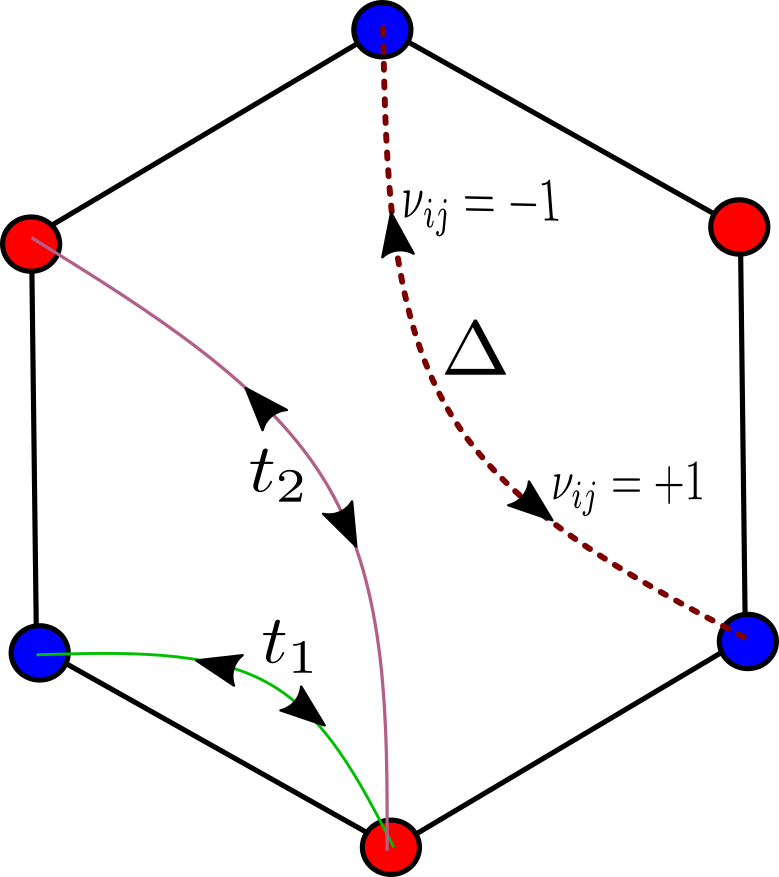
\includegraphics[width=0.6\columnwidth]{kmh.png}
\caption{A honeycomb cell with NN hopping $t_1$, NNN hopping $t_2$, intrinsic SOI $\Delta$, and $\nu_{ij} = \pm 1$ for clockwise and counterclockwise hoping.}
\label{fig1}
\vspace*{-6pt}
\end{figure}

Using the variational principle, it has been shown that the NN Coulomb interaction can be approximated by a renormalized local interaction $U =U_{00} - \bar{V}$, where $\bar{V}$ is a weighted average of the NN Coulomb interaction \cite{Schuler2013,Stepanov2017}. Thus, we only take into account the local Coulomb interaction in our total Hamiltonian and express the interaction part of the Hamiltonian in Eq. (\ref{Hint}) as
\begin{equation}
\hat{\mathcal{H}}_{\text{int}} \approx U\hat{d},
\end{equation}
where we define the doublon number operator $\hat{d} = \sum_{i=1} \hat{n}_{i\uparrow}\hat{n}_{i\downarrow}$ with eigenvalues $d$. We denote the projection operator to the subspace of states with eigenvalue $d$, i.e., states with exactly $d$ double occupancies, by $\hat{P}_d$. We are interested in the strongly correlated regime $U\gg t_{1(2)}$ at half-filling. In such a strong-coupling limit any state with a nonzero number of double occupancies ($d \neq 0$) has a much larger energy than those with no double occupancies ($d=0$). We obtain an effective Hamiltonian acting on the $d=0$ subspace by standard second-order perturbation theory in the hopping terms. Using the following relations,
\begin{align}
&\hat{c}_{i \tau}^\dagger \hat{c}_{i \tau'} = \frac{1}{2} (n_{i \uparrow} + n_{i \downarrow})\delta_{\tau \tau'}  + \bs{S}_i\cdot\bs{\tau}_{\tau', \tau}, \label{SpinOperatorInv1}\\
&\hat{c}_{i \tau} \hat{c}_{i \tau'}^\dagger = \frac{1}{2} (2 - n_{i \uparrow} - n_{i \downarrow}) \delta_{\tau \tau'} - \bs{S}_i\cdot\bs{\tau}_{\tau, \tau'}, \label{SpinOperatorInv2}
\end{align}
we find the spin Hamiltonian for 2D AFM Mott insulators,
\begin{align}
\label{MKMHeff0}
H_{\text{S}} =& J_{1}\sum_{\langle i,j \rangle} \bs{S}_i\cdot\bs{S}_j + J_{2}\sum_{\langle \langle i,j \rangle \rangle} \bs{S}_i\cdot\bs{S}_j,  \n \\
&+ \sum_{\langle \langle i,j \rangle \rangle} \bs{S}_i \bs{\Gamma}_{ij} \bs{S}_j +\sum_{\langle \langle i,j \rangle \rangle} \bs{D}_{ij}\cdot \bs{S}_i \times \bs{S}_j,
\end{align}
with the following spin-spin interactions,
\begin{subequations}
\label{spin-para}
\begin{align}
&J_{1(2)} = \frac{2t_{1(2)}^2}{U}, \\
&\bs{\Gamma}_{ij} =\frac{2\Delta^2}{U} \text{diag}(-1,-1,1),\\
&\bs{D}_{ij} = \frac{4 t_2 \Delta}{U}\nu_{ij}  \hat{\mathrm{e}}_z.
\end{align}
\end{subequations}
The first and second terms in the spin Hamiltonian, Eq. (\ref{MKMHeff0}), are the NN and NNN symmetric Heisenberg AFM exchange interactions, $J_{1(2)}>0$, respectively; the third term is the NNN anisotropic Heisenberg exchange interaction (XXZ-like term) arising from the intrinsic SOI, and finally, the last term is the intrinsic NNN DMI. The intrinsic SOI in Eq. (\ref{Hsoi}), leads to a DMI vector, $\bs{D}_{ij}$, perpendicular to the honeycomb plane. It can also be shown that the Rashba SOI results in an in-plane DMI vector that is perpendicular to the lattice bonds.
For the sake of completeness, we explain shortly the effect of disorder by adding an on-site disorder potential $\sum_{i \tau} \varepsilon_i \hat{c}_{i \tau}^\dagger \hat{c}_{i \tau}$ in the Kane-Mele-Hubbard Hamiltonian Eq. (\ref{MKMH}), where $\varepsilon_i$ is an uncorrelated random variable. Following the above procedure, it can be shown that the spin interaction parameters are renormalized as $U^{-1} \rightarrow U/\left(U^2-(\epsilon_j-\epsilon_i)^2\right)$ \cite{Protopopov2018}. In the large $U$ limit, the effect of disorder is negligible and we thus ignore it in the rest of this Letter.


The terms in the spin Hamiltonian derived in Eq. (\ref{MKMHeff0}) have already been obtained phenomenologically \cite{Owerre2016} and confirmed experimentally \cite{Chen2018}. To the best of our knowledge, this is the first microscopic derivation of the complete spin Hamiltonian $\hat{H}_{\text{S}}$ from the microscopic Kane-Mele-Hubbard model.
This Hamiltonian has interesting features and exotic phases like, the existence of magnon spin Nernst effect in collinear AFM layers \cite{Cheng2016, PhysRevLett.117.217203}, topological magnon insulator phase \cite{Owerre2016, Elyasi2018, Chen2018}, spin Hall effects of Weyl magnons \cite{Zyuzin2018, Sekine2016} magnonic Floquet topological insulators, spin density wave \cite{Mulder2010}, chiral and topological gapped spin liquid phases \cite{Vaezi}. Ultrafast control of DMI and exchange interaction by laser pulses enables engineering all these phenomena.



\textit{Laser illumination}.
The effect of laser irradiation is introduced in the Kane-Mele-Hubbard Hamiltonian, Eq. (\ref{MKMH}), via the Peierls substitution method \cite{Peierls1933}. The electric-field component of a polarized laser pulse is given by $\bs{E}(t) = \frac{E_0}{2}( e^{-i\omega t}\hat{\epsilon}+\mathrm{c.c.})$, where $E_0$ is the electric field amplitude, $\omega$ is the laser pulse frequency, and $\hat{\epsilon} = (\hat{\mathrm{e}}_x+i\lambda\hat{\mathrm{e}}_y)/\sqrt{1+\lambda^2}$ is the polarization unit vector with $\lambda= 0$ for linear polarization and $\lambda= \pm 1$ for right- and left handed polarizations.

It is more convenient to rewrite the noninteracting part of the Kane-Mele-Hubbard Hamiltonian, Eq. (\ref{MKMH}), as $\hat{T}_0=\hat{\mathcal{H}}_{\text{K}}+\hat{\mathcal{H}}_{\text{SOI}} = - \sum_{i,j , \tau, \tau'}
t_{ij}^{\tau\tau'} \hat{c}_{i \tau}^\dagger \hat{c}_{j \tau'}$, where the hopping amplitude is $t_{ij}^{\tau\tau'} = \delta_{\tau,\tau'}t_1$ for $i,j$ being NN and $t_{ij}^{\tau\tau'} = \delta_{\tau,\tau'}t_2 - i\Delta\nu_{ij}\sigma^z_{\tau, \tau'}$ for $i,j$ being NNN.
According to the Peierls substitution method, the hopping part of the Hamiltonian gain an extra phase $t_{ij}^{\tau\tau'}\rightarrow t_{ij}^{\tau\tau'} e^{{i e \bs{R}_{ij} \cdot \bs{A}(t)}}$, where $\bs{R}_{ij} = \bs{R}_i-\bs{R}_j$, $\bs{R}_i$ is the position of site $i$, $e$ is the electronic charge, and $\bs{A}$ is the vector potential of the laser pulse $\bs{A}(t) = \frac{1}{2}(\bs{A} e^{-i\omega t} + \mathrm{c.c.})$, with $\bs{A} = \frac{iE_0}{\omega}\hat{\epsilon}$.
The Peierls phase can be rewritten as $e\bs{R}_{ij}\cdot\bs{A} \equiv \alpha_{ij} e^{i \theta_{ij}}$, with $\alpha_{ij} = \pm|e\bs{R}_{ij}\cdot \bs{A}|$, in a such way that $\alpha_{ij}= -\alpha_{ji}$, $\theta_{ij}= \theta_{ji}$, and $\theta_{ij} \in \left[0,\pi\right)$.
Now, we use the Jacobi–-Anger expansion to rewrite the Peierls phase in the basis of its harmonics,
\begin{equation}
\label{JacobiAnger}
e^{ie\bs{R}_{ij}\cdot\bs{A}(t)} = \sum_m e^{i(\frac{\pi}{2}-\theta_{ij})m} \mathcal{J}_m(\alpha_{ij}) e^{im\omega t},
\end{equation}
where $\mathcal{J}_m(x)$ is the \textit{m}-th Bessel function of the first kind \cite{Kitamura2017}.

The total Hamiltonian in the presence of the laser field is time dependent through its hopping part, $\hat{H}(t) = \hat{T}(t) +  U\hat{d}$. Using Eq. (\ref{JacobiAnger}), we find $\hat{T}(t) = \sum_m \hat{T}_m e^{im \omega t}$, where $\hat{T}_m$ is the sum of all the \textit{m}-th Fourier mode of the hopping terms. We can additionally decompose $\hat{T}_m = \hat{T}_{-1,m}+\hat{T}_{0,m}+\hat{T}_{1,m}$, where $\hat{T}_{dm}(t)$ changes the doublon number by adding $d$ double occupancies, $\hat{T}_{dm}(t) = \sum_i \hat{P}_{i+d}\hat{T}_{m}(t)\hat{P}_i$. With this, we can write the hopping operator as
\begin{equation}
\hat{T}(t) = \sum_m (\hat{T}_{-1,m}+\hat{T}_{0,m}+\hat{T}_{1,m})e^{im\omega t},
\end{equation}

To find the renormalized spin Hamiltonian, we first derive an effective static Hamiltonian using the Floquet formalism \cite{Floquet1,2018NJPh...20i3022R,Floquet2}. To this end, we transform the original time-dependent Hamiltonian, $\hat{H}(t)$, by using a unitary transformation $\hat{U}(t) = e^{-i\hat{S}(t)}$,
\begin{equation}
\hat{H}'(t) = e^{i\hat{S}(t)} \left(\hat{H}(t)  -  i\partial_t \right) e^{-i\hat{S}(t)}.
\label{Htransformed}
\end{equation}
We perform the unitary transformation perturbatively in the hopping parameter. We can formally express $\hat{T}(t) = \eta \hat{T}(t)$, where $\eta$ plays the role of a bookkeeping parameter in the perturbation expansion. We expand $\hat{S}(t) = \sum_\nu \eta^\nu \hat{S}^{(\nu)}(t)$ and $\hat{H}'(t) = \sum_\nu \eta^\nu \hat{H}'^{(\nu)}(t)$. We require that the transformed Hamiltonian must have the same periodicity as the original time-dependent Hamiltonian. Thus the unitary transformation must have the same periodicity as the driven laser field so that $\hat{S}^{(\nu)}(t) = \sum_m e^{im\omega t}\hat{S}^{(\nu)}_m$. Additionally, we impose the transformed Hamiltonian to be block diagonal in the doublon number $d$. With the further requirement that $\hat{S}(t)$ does not contain block-diagonal terms we can uniquely determine the unitary transformation. Following the same procedure we used for the hopping operator, we write
\begin{equation}
\hat{S}^{(\nu)}(t) = \sum_{d \neq 0} \sum_m \eta^\nu \hat{S}^{(\nu)}_{d,m} e^{im\omega t},
\end{equation}
where $\hat{S}^{(\nu)}_{d,m}$ changes the double occupancy number by $d$. We expand the transformed Hamiltonian Eq. (\ref{Htransformed}) in power series of $\eta$ and determine $\hat{S}^{(\nu)}(t)$ iteratively in $\nu$ so that $\hat{H}'^{(\nu)}(t)$ is diagonal in the doublon number. After tedious, but straightforward calculations, the transformed Hamiltonian up to the second order in the hopping parameter is obtained $\hat{H}'(t)= \hat{T}'(t)+\text{U}\hat{d}$, where
\begin{align}
\label{transformedH}
&\hat{T}'(t) \approx  - \sum_m \hat{T}_{0,m}(t)e^{im\omega t} + \n \\
&+ \frac{1}{2}\sum_{mn} \left( \frac{\left[\hat{T}_{1,n}, \hat{T}_{-1,m-n} \right]}{\text{U}+n\omega} - \frac{\left[\hat{T}_{-1,n}, \hat{T}_{1,m-n} \right]}{\text{U}-n\omega} \right) e^{im\omega t}.
\end{align}
Now, we are in the situation that we can calculate the effective static Hamiltonian by time averaging of the transformed Hamiltonian $\hat{H}_{\text{eff}}=\hat{P}_0\hat{H}'(t)\hat{P}_0$, where $\hat{P}_0$ is the projection operator to the $d=0$ subspace.
After some algebra, the effective static Hamiltonian in terms of creation and annihilation operators is obtained,
\begin{align}
\hat{H}_{\text{eff}} &= - \sum_{i,j, \tau, \tau'} \left(t_{ij}^{\tau} t_{ji}^{\tau'} \sum_{n} \frac{\mathcal{J}_{n}^2(\alpha_{ij})}{\text{U}+n\omega} \right)  \hat{c}_{i \tau}^\dagger \hat{c}_{j \tau} \hat{c}_{j \tau'}^\dagger \hat{c}_{i \tau'}. \label{GeneralHeff}
\end{align}



Finally, the spin Hamiltonian at half-filling is obtained using the relations Eqs. (\ref{SpinOperatorInv1}) and (\ref{SpinOperatorInv2}):
\begin{align}
\label{MKMHeffw}
\tilde{H}_{\text{S}}(\omega) =& \tilde{J}_{1}\sum_{\langle i,j \rangle} \bs{S}_i\cdot\bs{S}_j + \tilde{J}_{2}\sum_{\langle \langle i,j \rangle \rangle} \bs{S}_i\cdot\bs{S}_j, \n \\
&+ \sum_{\langle \langle i,j \rangle \rangle} \bs{S}_i \tilde{\bs{\Gamma}}_{ij} \bs{S}_j +\sum_{\langle \langle i,j \rangle \rangle} \tilde{\bs{D}}_{ij}\cdot \bs{S}_i \times \bs{S}_j,
\end{align}
with the following renormalized spin interactions,
\begin{subequations}
\label{Renor-para}
\begin{align}
&\tilde{J}_{1(2),ij} = 2t_{1(2)}^2\sum_n\frac{\mathcal{J}_{n}^2(\alpha_{ij})}{\text{U}+n\omega}, \\
&\tilde{\bs{\Gamma}}_{ij} = 2\Delta^2 \text{diag}(-1,-1,1) \sum_n\frac{\mathcal{J}_{n}^2(\alpha_{ij})}{\text{U}+n\omega},\\
&\tilde{\bs{D}}_{ij} = 4 t_2 \Delta \sum_n\frac{\mathcal{J}_{n}^2(\alpha_{ij})}{\text{U}+n\omega} \nu_{ij} \hat{\mathrm{e}}_z.
\end{align}
\end{subequations}
All spin interaction parameters are renormalized by the same function, but $\alpha_{ij}$ differs for NN and NNN parameters. Thus, the ratios between the NN and NNN renormalized parameters are different than those of non-perturbed parameters. The renormalized spin interactions presented in Eq. (\ref{Renor-para}) are helicity independent.

\begin{figure}[t]
\centering
\vspace{-1.3cm}
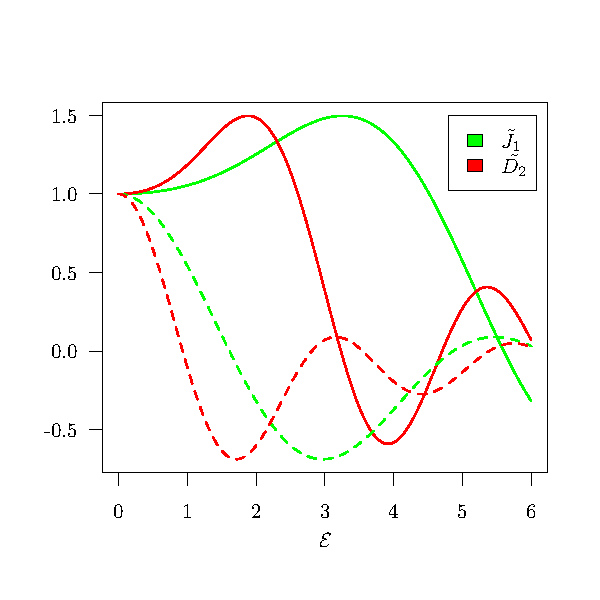
\includegraphics[width=\columnwidth]{NNvsNNN1_big_margin.pdf}
\vspace{-1cm}
\caption{Dimensionless exchange interaction (green lines) and DMI (red lines) as a function of the Floquet parameter $\mathcal{E} = \frac{eaE_0}{\omega}$, for two laser frequencies $\omega = 4$ (solid lines) and $\omega = 14$ (dashed lines).}
\label{fig2}
\end{figure}

Figure \ref{fig2}, shows the dependence of dimensionless NN exchange interaction $\tilde{J}_{1,ij}/J_{1,ij}$ and dimensionless NNN DMI $\tilde{D}_{ij}/D_{ij}$ on the Floquet parameter $\mathcal{E} = \frac{e a E_0}{\omega}$, where $a$ is the lattice constant. We show this dependence for two different laser pulse frequencies. We set $\hbar = 1$ and $t_1=1$ and measure energy in units of $t_1$ and frequency in units of $\frac{t_1}{\hbar}$. The results are obtained for material parameters $t_2=0.1$ and $\text{U} = 10$. Figure \ref{fig2}, shows that it is possible not only to change the sign and amplitude of the exchange interaction as already reported in Ref. \cite{Mentink2015} but it is possible to change the sign and amplitude of the intrinsic DMI. More importantly, the ratio $\tilde{J}_{1,ij}/\tilde{D}_{ij}\neq J_{1,ij}/D_{ij}$ can be tuned by laser excitations which is responsible for ultrafast photoinduced spin dynamics and magnon scattering phenomena.

Eqs. (\ref{MKMHeffw}) and (\ref{Renor-para}) explicitly show that the spin Hamiltonian in the presence of a time-dependent external field can be effectively written as $\tilde{H}_{\text{S}}=H_{\text{S}}+g_{\alpha \beta i j} S^\alpha_i S^\beta_j E^{\alpha} E^{*\beta} $, where $\alpha$ and $\beta$ represent the spatial component of vectors, $i$ and $j$ refer to the lattice site, and $g$ is the opto-magnetic coupling tensor which can be read from Eqs. (\ref{Renor-para}). Thus, the dielectric permittivity tensor which determines the optical properties of the medium, is given by $\varepsilon_{\alpha \beta}=\partial^2 \tilde{H}_{\text{S}}/\partial E^{\alpha}\partial E^{*\beta}$. This opto-magnetic effect described by the dielectric permittivity $\varepsilon$, can be detected by measuring the intensity of the scattered light $I_{\mathrm{sc}} \propto (\varepsilon_{\alpha \beta} E_0)^2$ \cite{Demokritov1985}.

In ultrafast spin dynamics experiments, very intense laser pulses are used and one might think on how heating might affect the validity of our approach. Recent theoretical \cite{Rudner2019,PhysRevB.97.014311} and experimental \cite{PhysRevA.96.053602} works show that the energy absorption rate is suppressed exponentially for high frequency laser pulses $\omega/W\gg 1$, where $W\propto t_1$ is the fermionic bandwidth, which is the case in ultrafast experiments with optical laser pulses. Thus, rapidly driven systems have a very long prethermalization period and this implies that the evolution of these systems in the presence of short laser pulses can be described by our formalism safely.



The possibility of ultrafast optical modification of the exchange interactions in the bulk of iron oxides has been recently reported \cite{Mikhaylovskiy2015}. We hope that our work will stimulate new experiments on measuring both exchange interaction and DMI in novel 2D magnetic systems.

In summary, we have investigated the effect of polarized and intense high-frequency laser pulses on 2D canted antiferromagnetic Mott insulators using Floquet theory. We have found that both sign and amplitude of the ratio between the exchange interaction and DMI is changed in honeycomb lattices irrespective to the helicity of laser pulses. Our calculations open a new way to ultrafast and energy-efficient control of spins and engineering of topological objects and topological properties of 2D van der Waals magnetic materials.


\section*{Acknowledgments}
The research leading to these results was supported by the European Research Council via Advanced Grant No. 669442, ``Insulatronics,'' and by the Research Council of Norway through its Centres of Excellence funding scheme, Project No. 262633, ``QuSpin.''


%\begin{thebibliography}
\bibliographystyle{apsrev4-1}
\bibliography{paper}
%\end{thebibliography}

\end{document}


